\documentclass[11pt,a4paper]{article}
\usepackage[utf8]{inputenc}
\usepackage[T1]{fontenc}
\usepackage[brazil]{babel}
\usepackage{amsmath,booktabs,graphicx,geometry}
\usepackage[authoryear,round]{natbib}
\usepackage{hyperref}
\geometry{margin=2.5cm}
\hypersetup{colorlinks=true,linkcolor=blue,urlcolor=blue,citecolor=blue}

\title{Ganhar a vaga preferida atrai o especialista?\\
Efeito local no cutoff de seleção do Programa Mais Médicos Especialistas}
\author{Versão de trabalho}
\date{9 de setembro de 2026}

\begin{document}
\maketitle

\begin{abstract}
Este trabalho estima se obter marginalmente uma vaga de primeira opção aumenta
a adesão e a presença posterior de especialistas no estabelecimento escolhido
no Programa Mais Médicos Especialistas (PMM-E). Usamos apenas publicações
oficiais de classificação, homologação e participantes ativos. A amostra
principal compara, dentro do mesmo curso, estabelecimento, chamada e modalidade
de ampla concorrência, o último candidato selecionado e o primeiro não
selecionado quando as pontuações diferem em exatamente um ponto; empates são
excluídos porque dependem de critérios de desempate não publicados. Em 36 pares
de 2025, ganhar a vaga elevou a homologação no mesmo curso--CNES em 63,9 pontos
percentuais (intervalo convencional de 47,4 a 80,4; teste exato pareado com $p$
abaixo de 0,000001) e a presença ativa no mesmo curso--CNES em 12 de agosto de
2026 em 33,3 pontos percentuais (13,5 a 53,1; $p$ exato de 0,0042). O placebo
imediatamente abaixo do cutoff é nulo, com $-$3,3 e 0,0 pontos percentuais;
janelas alternativas de gap e a exclusão sucessiva de cada curso e de cada
unidade da federação preservam sinal e ordem de magnitude. Em 11 pares do ciclo
2 de 2026, a presença ativa aumenta 36,4 pontos percentuais, com teste exato
impreciso ($p$ de 0,125). Como a pontuação é discreta e o protocolo é
retrospectivo, o resultado é um efeito local condicional à comparabilidade entre
candidatos separados por um ponto, com grau de rigor moderado. O desenho informa
a conversão de uma alocação em ingresso e presença; não identifica o efeito da
bolsa, do Índice de Vulnerabilidade Social (IVS), do PMM-E sobre o estoque
municipal, a decisão de se inscrever, a retenção contínua, a produção
assistencial ou desfechos de saúde.
\end{abstract}

\section{Introdução}
\label{sec:introducao}

A distribuição territorial de especialistas não depende apenas da existência de
vagas. Ela depende de o médico aceitar uma oportunidade concreta e de
efetivamente aparecer no local em que foi alocado. Essa margem é a do
\emph{matching} entre candidato e vaga, e ela é frequentemente tratada como
resolvida nas avaliações de políticas de provimento, que costumam comparar
territórios ou coortes já alocadas.

O PMM-E permite observar essa margem de forma direta. Dentro de cada célula
curso--estabelecimento, os candidatos declaram preferências e são ordenados por
pontuação. Alguns ganham a vaga de primeira opção; outros ficam imediatamente
abaixo do limite de seleção. Este trabalho explora essa fronteira administrativa
para perguntar se o acesso marginal à vaga preferida se converte em adesão e em
presença posterior naquele estabelecimento.

A contribuição é deliberadamente estreita. Não estimamos preferências
estruturais, produção assistencial, internações, exames nem o estoque geral de
médicos do município. Também não identificamos o efeito da remuneração adicional
associada ao IVS: o IVS público não reproduz a faixa administrativa anunciada
nem gera primeiro estágio estável, e essa rota foi arquivada (Apêndice
\ref{sec:rotas}). Examinamos apenas o ponto em que a regra muda a alocação entre
dois candidatos quase idênticos do ponto de vista do processo seletivo.

Duas palavras precisam de definição imediata, porque organizam toda a leitura.
\textbf{Atração} significa aqui atração realizada, isto é, a conversão de uma
preferência declarada em ingresso e presença; não significa geração de novas
candidaturas, já que a amostra começa depois da inscrição. \textbf{Retenção}
significa presença observada em uma data específica; não significa permanência
contínua, duração do vínculo nem tempo até a saída.

\section{Literatura e posicionamento}
\label{sec:literatura}

A escolha locacional de médicos é usualmente modelada como maximização de
retornos líquidos entre localidades, com diferenciais compensatórios por
desamenidades \citep{roback1982}. Aplicações empíricas modernas estimam
equilíbrios espaciais com salários, aluguéis e amenidades \citep{diamond2016} e
associam a escassez rural de médicos à organização da formação e à
infraestrutura produtiva \citep{moehling2020}. Para o Brasil,
\citet{costa2024} estimam um modelo de escolha discreta com coeficientes
aleatórios para generalistas formados entre 2001 e 2013: proximidade ao local de
nascimento ou de formação é determinante, e os contrafactuais favorecem políticas
de formação e origem em relação a incentivos puramente financeiros.
\citet{sivey2012} estimam, com modelos de utilidade aleatória, a disposição a
aceitar postos no interior entre médicos em início de carreira. Essa literatura
descreve preferências sobre localidades; ela não isola o que ocorre quando duas
pessoas com a mesma preferência declarada recebem decisões administrativas
diferentes.

A literatura de incentivos de provimento avalia programas que condicionam bolsa,
bônus ou perdão de dívida ao serviço em áreas desassistidas.
\citet{barnighausen2009} sintetizam 43 programas em dez países e mostram
heterogeneidade grande de cumprimento. \citet{gravelle2018} decompõem o efeito
de bônus rurais em entradas e saídas de clínicos gerais. \citet{pathman2004}
acompanham coortes de programas estaduais nos Estados Unidos e documentam
permanência alta durante a obrigação e queda rápida depois dela.
\citet{russell2021} estimam determinantes do tempo até a evasão em municípios
rurais australianos. Esses trabalhos medem retenção como duração; o desenho
público disponível aqui mede presença em uma data e, por isso, não é comparável
a eles nesse ponto.

No Brasil, as avaliações do Programa Mais Médicos usam bases administrativas do
DATASUS para medir consultas e internações sensíveis \citep{fontes2018},
exploram regras de pontuação do edital com estudo de evento \citep{carrillo2019}
e usam o painel mensal do Cadastro Nacional de Estabelecimentos de Saúde (CNES)
para acompanhar um choque abrupto de oferta \citep{sliwa2024}. Essas avaliações
tratam de generalistas na atenção primária e de desfechos assistenciais
agregados. O PMM-E, criado pela Lei 15.233/2025, dirige-se a especialistas e
opera por um edital centralizado com preferências declaradas, o que aproxima o
programa dos mercados de \emph{matching} médico estudados por
\citet{roth1984} e \citet{agarwal2015}.

Nosso posicionamento é o seguinte. As duas primeiras literaturas estimam como
atributos de localidade e incentivos deslocam escolhas; a terceira estima efeitos
agregados de programas de provimento; a quarta modela o mecanismo de alocação.
Este trabalho isola um elo intermediário que essas abordagens normalmente tomam
como dado: dada a candidatura e a preferência declarada, quanto a própria decisão
de alocação altera a adesão administrativa e a presença posterior do
especialista no estabelecimento pretendido. É uma quantidade local e pequena em
escopo, mas identificada em um contraste institucionalmente bem definido e
estimada apenas com publicações abertas.

\section{Contexto institucional e hipótese identificadora}
\label{sec:contexto}

No PMM-E, o candidato informa preferências ordenadas de curso e estabelecimento
e é classificado por pontuação de barema dentro de cada modalidade de inscrição.
Em cada célula curso--CNES, a última posição contemplada recebe a alocação e a
posição seguinte não a recebe naquela chamada. O edital prevê critérios de
desempate por mesma unidade da federação e maior idade, mas os campos
individuais que operacionalizam esses critérios não constam das listas públicas.

A hipótese identificadora é que candidatos da mesma célula curso--CNES, da mesma
chamada, ambos em ampla concorrência, ambos com aquela vaga como primeira opção
e separados por exatamente um ponto teriam resultados potenciais comparáveis na
ausência da alocação. Sob essa hipótese, a mudança de tratamento no limite de
seleção identifica um efeito local de ganhar a vaga de primeira opção.

Três qualificações precisam ficar explícitas desde já.

Primeiro, esta hipótese é mais forte do que a continuidade usada em uma
regressão descontínua com \emph{running variable} efetivamente contínua. A
pontuação é discreta e a amostra principal observa apenas um valor de escore de
cada lado de cada cutoff. Não é possível fazer a diferença de escore tender
arbitrariamente a zero, de modo que a identificação depende da hipótese
substantiva de que um ponto de barema não desloca, por outro canal, a propensão
a homologar ou a permanecer.

Segundo, o desenho não é um sorteio. A pontuação reflete experiência e
qualificação declaradas, e a comparabilidade entre os dois lados é uma hipótese,
não um fato garantido pelo procedimento.

Terceiro, o cutoff é específico de cada vaga, e não um limiar único aplicado a
toda a população. O contraste é interno à célula e à chamada, e o estimando é um
efeito local médio entre os pares marginais efetivamente observados.

Por essas razões, o resultado é descrito ao longo do texto como \emph{efeito
local condicional à comparabilidade}, com grau de rigor moderado, e nunca como
regressão descontínua convencional ou como experimento aleatorizado.

\section{Dados e método}
\label{sec:metodo}

\subsection{Fontes}

Todas as informações vêm de publicações oficiais já disponíveis: os resultados de
classificação e alocação das chamadas do ciclo 1 de 2025, as listas de
homologação correspondentes, o resultado final da segunda chamada do ciclo 2 de
2026 e um retrato nominal dos participantes ativos com data de referência de 12
de agosto de 2026. As seis entradas têm hash SHA-256 congelado no protocolo do
módulo. Nomes são processados apenas em memória para a ligação exata entre
publicações; nenhum identificador individual, nenhum hash de candidato e nenhum
par reidentificável é gravado nos artefatos.

\subsection{Amostra}

Para cada célula curso--CNES, tomamos o último candidato alocado e o primeiro
não alocado, exigindo cumulativamente que: (i) ambos tenham declarado aquela
vaga como primeira opção; (ii) ambos concorram em ampla concorrência; (iii)
exista exatamente uma pessoa em cada posição adjacente; (iv) a pontuação do
selecionado supere a do não selecionado em exatamente um ponto; e (v) o
tratamento efetivamente mude entre as duas posições, caracterizando um corte
\emph{sharp} no ranking. Linhas explicitamente rotuladas como sub judice são
descartadas nas publicações que trazem esse marcador.

O critério (iv) é o que separa este recorte do diagnóstico anterior, que
misturava empates e diferenças maiores de pontuação. Como os empates dependem
dos desempates não publicados por unidade da federação e idade, eles não entram
na análise causal e são reportados apenas de forma descritiva.

A Tabela \ref{tab:suporte} mostra a construção do suporte. Em 2025, restam 30
pares na primeira chamada e 6 na segunda, totalizando 36 pares; 76 pares
empatados são excluídos. Não há violações do sentido do gap em nenhuma chamada,
não há nomes repetidos entre os pares principais e não há células repetidas entre
as duas chamadas de 2025.

\begin{table}[htbp]
\centering
\footnotesize
\caption{Construção do suporte amostral no limite de seleção}
\label{tab:suporte}
\begin{tabular}{lrrrrrrr}
\toprule
Ciclo e chamada & Pares & Cutoff & Gap de 1 & Empates & Violações & Placebo & Placebo \\
 & adjacentes & (AC) & ponto (AC) & excluídos & do gap & abaixo & acima \\
\midrule
2025, ciclo 1, chamada 1 & 136 & 123 & 30 & 48 & 0 & 20 & 3 \\
2025, ciclo 1, chamada 2 & 57 & 53 & 6 & 28 & 0 & 10 & 2 \\
2026, ciclo 2, chamada 2 & 56 & 50 & 11 & 26 & 0 & 8 & 4 \\
\bottomrule
\end{tabular}

\vspace{2pt}
\begin{minipage}{0.94\textwidth}
\footnotesize \textit{Nota:} AC indica ampla concorrência. ``Cutoff (AC)'' conta
os pares adjacentes em que o corte no ranking é \emph{sharp} e ambos os
candidatos concorrem em ampla concorrência. As colunas de placebo contam pares
com gap de um ponto em que a alocação não muda entre as duas posições.
\end{minipage}
\end{table}

\subsection{Tratamento e hierarquia de desfechos}

O tratamento é ganhar a alocação da vaga de primeira opção naquela chamada.

Os desfechos são hierarquizados. A \textbf{homologação no mesmo curso--CNES} é
um desfecho de processo: mede a conversão administrativa imediata, mas está
próxima da própria elegibilidade criada pela seleção, de modo que um efeito
grande não é, por si só, a novidade substantiva. O \textbf{desfecho substantivo
principal} é estar ativo no mesmo curso--CNES em 12 de agosto de 2026, definido
para todos os candidatos do par e incondicional à homologação; por ser posterior
e incondicional, ele preserva o efeito total da alocação em vez de selecionar
apenas quem já entrou. Como sensibilidade, medimos homologação e atividade em
qualquer local do programa, o que permite verificar se o candidato não
selecionado ingressou por outra vaga.

A ausência no retrato de 12 de agosto de 2026 significa apenas não estar ativo
naquela data. Ela não informa data de saída, duração do vínculo nem permanência
contínua, e não deve ser lida como taxa de evasão.

\subsection{Estimação e inferência}

Para cada par, calculamos a diferença binária entre o candidato acima e o
candidato abaixo do limite de seleção. A estimativa é a média dessas diferenças
pareadas. Reportamos o teste exato bicaudal condicionado aos pares discordantes
e, como descrição de incerteza, um intervalo t pareado explicitamente rotulado
como convencional.

O teste exato é mais transparente do que depender apenas de aproximações
assintóticas com 36 pares, mas ele não torna a atribuição aleatória: sua validade
causal continua condicionada à hipótese de comparabilidade local da Seção
\ref{sec:contexto}. Pela mesma razão, não usamos agrupamento por valor do escore
como se isso corrigisse especificação incorreta com apenas um ponto de massa de
cada lado.

Os diagnósticos são: pares de placebo imediatamente abaixo e imediatamente acima
do cutoff, onde a alocação não muda; janelas alternativas de gap positivo de até
dois pontos e de qualquer tamanho; desfechos em qualquer local; exclusão
sucessiva de cada curso e de cada unidade da federação; e replicação no ciclo 2
de 2026.

\subsection{Protocolo}

O protocolo do módulo foi congelado depois que uma análise anterior de pares
adjacentes, com 423 pares nas quatro publicações, já havia observado os
desfechos. Portanto, este é um \textbf{protocolo retrospectivo}, e não um
pré-registro prospectivo. O recorte estrito foi definido para eliminar empates e
gaps heterogêneos, e não escolhido depois de comparar resultados alternativos,
mas o leitor deve tratar a estimativa como retrospectiva ao ponderar a evidência.

\section{Resultados}
\label{sec:resultados}

\subsection{Resultado principal de 2025}

A Tabela \ref{tab:principal} apresenta o resultado principal nos 36 pares de
2025. Ganhar marginalmente a vaga de primeira opção elevou a homologação no
mesmo curso--CNES em 63,9 pontos percentuais e a presença ativa no mesmo
curso--CNES em 33,3 pontos percentuais. Entre os 36 pares, 23 são discordantes e
todos favoráveis no desfecho de homologação; no desfecho de presença ativa, 14
são favoráveis e 2 contrários.

\begin{table}[htbp]
\centering
\small
\caption{Efeito local da alocação de primeira opção, 36 pares de 2025}
\label{tab:principal}
\begin{tabular}{lrrrrcr}
\toprule
Desfecho & Selec. & Não selec. & Diferença & EP & IC95\% convencional & $p$ exato \\
 & (\%) & (\%) & (p.p.) & (p.p.) & (p.p.) & \\
\midrule
Homologação no mesmo curso--CNES & 63,9 & 0,0 & 63,9 & 8,1 & [47,4; 80,4] & $<$0,000001 \\
Ativo no mesmo curso--CNES & 41,7 & 8,3 & 33,3 & 9,8 & [13,5; 53,1] & 0,0042 \\
Homologação em qualquer local & 63,9 & 5,6 & 58,3 & 9,2 & [39,6; 77,1] & 0,0000057 \\
Ativo em qualquer local & 50,0 & 16,7 & 33,3 & 12,0 & [9,1; 57,6] & 0,0169 \\
\bottomrule
\end{tabular}

\vspace{2pt}
\begin{minipage}{0.94\textwidth}
\footnotesize \textit{Nota:} diferenças pareadas entre o candidato imediatamente
acima e o imediatamente abaixo do limite de seleção, em pares de ampla
concorrência, primeira opção e gap de exatamente um ponto. O intervalo t pareado
é convencional e não corrige a discretização do escore. O teste exato é bicaudal
e condicionado aos pares discordantes. ``Ativo'' refere-se ao retrato de 12 de
agosto de 2026.
\end{minipage}
\end{table}

A homologação mostra conversão administrativa forte, mas seu zero entre os não
selecionados é em parte esperado pela estrutura da chamada, já que a homologação
naquele local pressupõe a alocação naquele local. O resultado substantivamente
mais informativo é a presença posterior: candidatos marginalmente selecionados
têm probabilidade 33,3 pontos percentuais maior de aparecer ativos naquele
curso--CNES no retrato de 12 de agosto de 2026.

Os desfechos em qualquer local do programa mostram que o efeito não é apenas uma
troca mecânica de endereço entre participantes que entrariam de qualquer forma:
a diferença é de 58,3 pontos percentuais em homologação e de 33,3 pontos
percentuais em atividade. A recolocação dos não selecionados em outras vagas é
parcial, e não integral, dentro do horizonte observado.

Separando as chamadas de 2025, a diferença de homologação é de 60,0 pontos
percentuais nos 30 pares da primeira chamada e de 83,3 pontos percentuais nos 6
pares da segunda; a diferença de presença ativa é de 33,3 pontos percentuais em
ambas. A segunda chamada tem pares insuficientes para inferência isolada e é
reportada apenas por transparência.

\subsection{Placebos}

A Tabela \ref{tab:placebos} reporta os placebos. Entre os 30 pares de não
selecionados separados por um ponto imediatamente abaixo do cutoff, onde a
alocação não muda, a diferença é de $-$3,3 pontos percentuais em homologação e
de 0,0 ponto percentual em presença ativa, ambas com teste exato de 1,000. O
salto principal, portanto, não reaparece onde o tratamento não muda.

O placebo imediatamente acima do cutoff tem apenas 5 pares e produz $-$20,0
pontos percentuais em ambos os desfechos, com teste exato de 1,000. Com esse
número de pares, o exercício não é informativo sobre precisão; ele é mantido por
transparência, e não como teste decisivo.

\begin{table}[htbp]
\centering
\small
\caption{Placebos com gap de um ponto onde a alocação não muda, 2025}
\label{tab:placebos}
\begin{tabular}{llrrr}
\toprule
Placebo & Desfecho & Pares & Diferença (p.p.) & $p$ exato \\
\midrule
Imediatamente abaixo & Homologação no mesmo curso--CNES & 30 & $-$3,3 & 1,000 \\
Imediatamente abaixo & Ativo no mesmo curso--CNES & 30 & 0,0 & 1,000 \\
Imediatamente abaixo & Homologação em qualquer local & 30 & 6,7 & 0,6875 \\
Imediatamente abaixo & Ativo em qualquer local & 30 & $-$3,3 & 1,000 \\
Imediatamente acima & Homologação no mesmo curso--CNES & 5 & $-$20,0 & 1,000 \\
Imediatamente acima & Ativo no mesmo curso--CNES & 5 & $-$20,0 & 1,000 \\
\bottomrule
\end{tabular}
\end{table}

\subsection{Sensibilidade de gap e leave-one-out}

A Tabela \ref{tab:gap} amplia a janela de pontuação. Com gap positivo de até dois
pontos, o efeito é de 58,1 pontos percentuais em homologação e de 35,1 pontos
percentuais em presença ativa, em 74 pares. Com qualquer gap positivo, o efeito é
de 58,0 e 36,0 pontos percentuais, em 100 pares. Sinal e ordem de magnitude não
dependem da janela escolhida.

A última linha da Tabela \ref{tab:gap} reporta os 76 pares empatados apenas como
descrição. Eles voltam a depender dos desempates não observados por unidade da
federação e idade e, por isso, não sustentam leitura causal, ainda que as
diferenças brutas sejam grandes.

\begin{table}[htbp]
\centering
\small
\caption{Janelas alternativas de gap de pontuação, 2025}
\label{tab:gap}
\begin{tabular}{lrrr}
\toprule
Recorte & Pares & Homologação (p.p.) & Ativo (p.p.) \\
\midrule
Gap de exatamente 1 ponto (principal) & 36 & 63,9 & 33,3 \\
Gap positivo de até 2 pontos & 74 & 58,1 & 35,1 \\
Qualquer gap positivo & 100 & 58,0 & 36,0 \\
Empates (descritivo, não causal) & 76 & 64,5 & 43,4 \\
\bottomrule
\end{tabular}

\vspace{2pt}
\begin{minipage}{0.9\textwidth}
\footnotesize \textit{Nota:} desfechos medidos no mesmo curso--CNES. A última
linha é contaminada por critérios de desempate não publicados e é reportada
apenas como descrição.
\end{minipage}
\end{table}

Excluindo sucessivamente cada um dos 12 cursos e cada uma das 11 unidades da
federação presentes na amostra principal, em 23 exclusões, a diferença de
homologação permanece entre 58,1 e 71,0 pontos percentuais e a diferença de
presença ativa permanece entre 27,3 e 38,7 pontos percentuais. Nenhum curso e
nenhuma unidade da federação isolada cria ou inverte o resultado.

\subsection{Replicação de 2026}

Na segunda chamada do ciclo 2 de 2026, 11 pares atendem ao mesmo critério
estrito. A diferença de presença ativa no mesmo curso--CNES é de 36,4 pontos
percentuais, próxima da estimativa de 2025. O intervalo convencional vai de 2,5 a
70,3 pontos percentuais, mas o teste exato é de 0,125, porque há apenas 4 pares
discordantes. A classificação correta é replicação direcional consistente, porém
imprecisa: ela reforça a plausibilidade externa da direção do efeito e não
adiciona precisão.

A Figura \ref{fig:a8} resume o conjunto: as duas estimativas principais de 2025,
os dois placebos imediatamente abaixo do cutoff e a replicação de 2026.

\begin{figure}[htbp]
\centering
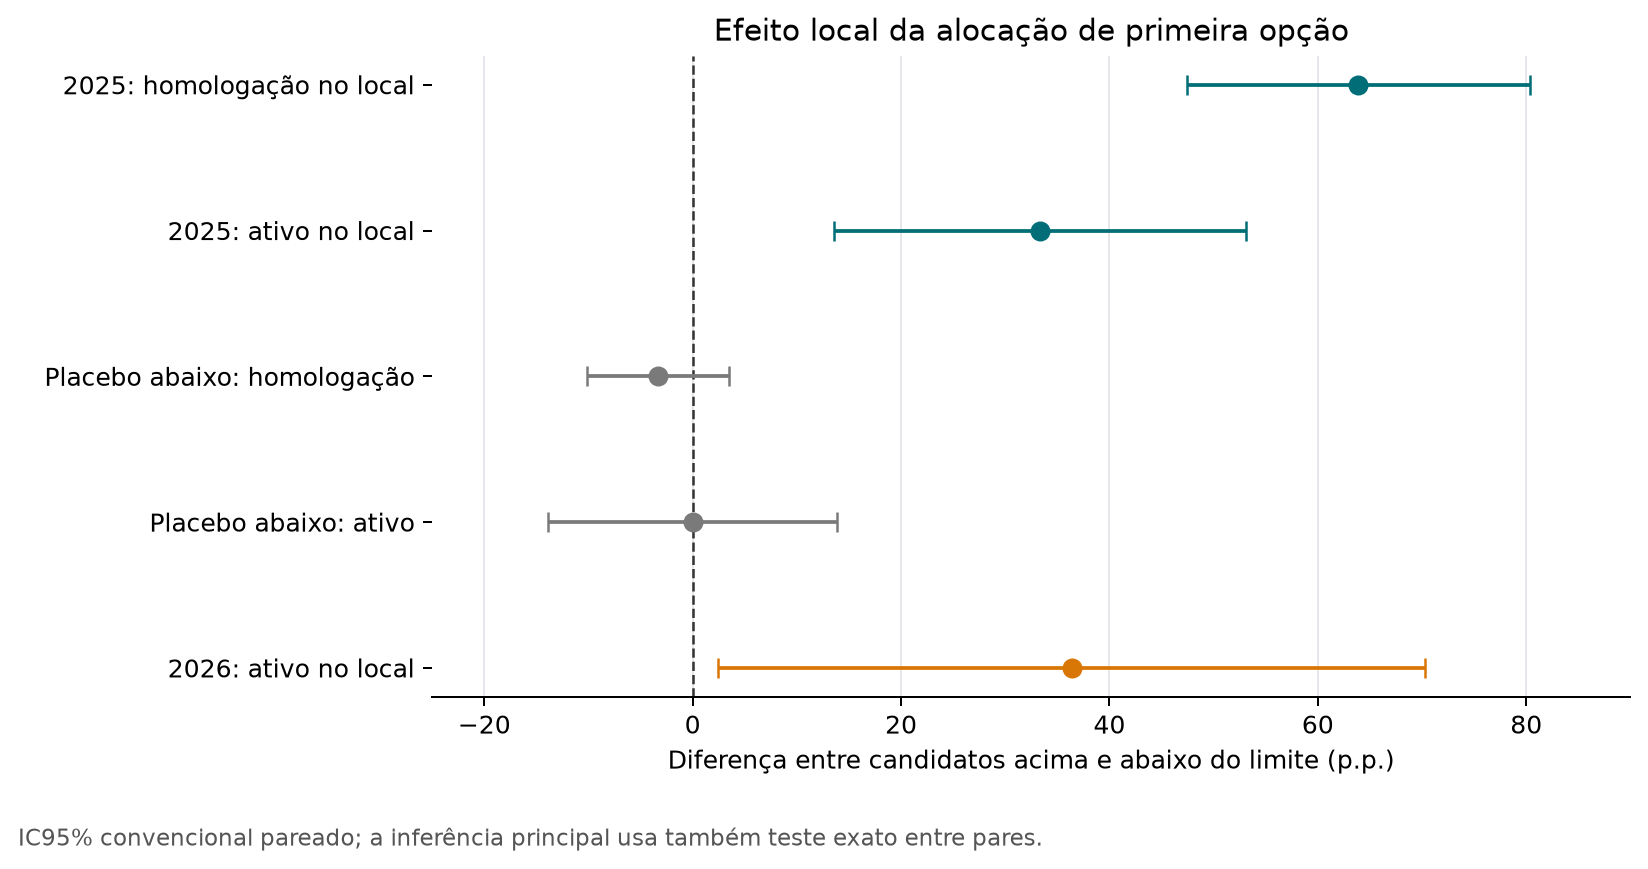
\includegraphics[width=0.94\textwidth]{output/tema_trabalho/A8_figura_01_efeitos_cutoff_escore.png}
\caption{Efeito local da alocação de primeira opção. Pontos são diferenças
pareadas entre candidatos imediatamente acima e imediatamente abaixo do limite
de seleção; as barras são intervalos t pareados convencionais de 95\%, que não
corrigem a discretização do escore. A inferência principal usa também o teste
exato entre pares discordantes.}
\label{fig:a8}
\end{figure}

\section{Discussão, alcance e limitações}
\label{sec:discussao}

Os resultados indicam que o \emph{matching} administrativo importa. Para
candidatos no limite da mesma vaga preferida, receber efetivamente a alocação
aumenta substancialmente a chance de o especialista aparecer ativo naquele
estabelecimento em data posterior. Essa é uma margem de desenho de programa:
quantas vagas abrir por célula, como ordenar preferências e como tratar
chamadas subsequentes afetam onde o profissional efetivamente aparece, e não
apenas o registro formal da seleção. Em políticas de base territorial, o
desenho da alocação é parte do instrumento, e não um detalhe operacional
\citep{kline2014}.

O alcance do resultado é limitado de forma deliberada. O desenho \textbf{não}
identifica: o efeito da bolsa ou do adicional associado ao IVS; o efeito do
IVS; o efeito do PMM-E sobre o estoque municipal de especialistas; o efeito
sobre a decisão de se inscrever, pois todos os comparados já são candidatos;
retenção contínua ou duração até a saída; produção assistencial, filas ou
desfechos de saúde. Nenhuma dessas quantidades pode ser inferida das estimativas
aqui reportadas.

Quatro limitações organizam a leitura. Primeiro, a pontuação é discreta, com
apenas um ponto de massa de cada lado do cutoff, e um ponto de barema pode
capturar experiência ou qualificação correlacionadas com adesão; a
comparabilidade local é uma hipótese não integralmente testável. Segundo, a
amostra principal tem 36 pares, o que limita a precisão e impede
heterogeneidades confiáveis por território, curso ou região. Terceiro, a ligação
entre publicações usa nome normalizado exato e a chave curso--CNES; embora a
unicidade tenha sido auditada e nenhum nome se repita entre os pares principais,
não há identificador pseudonimizado estável. Quarto, o recorte estrito foi
congelado depois que a análise anterior já havia aberto os desfechos, de modo que
o protocolo é retrospectivo.

Há ainda uma limitação de medida. O desfecho substantivo é um retrato em 12 de
agosto de 2026. Ele não permite reconstruir curvas de sobrevivência, porque a
data de início só é observada entre quem segue ativo, o que selecionaria
sobreviventes. Por isso o texto fala em presença, e não em permanência.

O gradiente territorial descritivo do Apêndice \ref{sec:territorio} explica por
que a alocação importa: a atração administrativa realizada é sistematicamente
menor no interior remoto do que em células metropolitanas. Esse gradiente é
associativo e não deve ser fundido ao estimando causal. Do mesmo modo, a
evidência longitudinal do CNES no Apêndice \ref{sec:cnes} mede outro objeto
--- o estoque cadastral municipal por curso --- e não pode ser usada para
confirmar o resultado local do cutoff.

\section{Conclusão}
\label{sec:conclusao}

Sob a hipótese de comparabilidade local entre candidatos separados por um ponto,
ganhar marginalmente a vaga de primeira opção aumentou a homologação no mesmo
curso--CNES em 63,9 pontos percentuais e a presença ativa posterior naquele
mesmo curso--CNES em 33,3 pontos percentuais. O efeito aparece nas duas chamadas
de 2025, não se reproduz no placebo imediatamente abaixo do cutoff, permanece
estável em janelas alternativas de gap e na exclusão sucessiva de cursos e
unidades da federação, e tem direção semelhante em uma pequena replicação de
2026.

Para um trabalho curto, a conclusão deve permanecer nesse nível. O estudo oferece
evidência causal local sobre alocação, adesão e presença, com grau de rigor
moderado, \emph{running variable} discreta e protocolo retrospectivo. A análise
territorial descritiva explica a relevância do problema, mas não integra o
estimando causal. A avaliação do adicional de bolsa pelo IVS e os desfechos de
produção assistencial permanecem fora do escopo e exigiriam, respectivamente, a
reconstrução da regra administrativa e portões próprios de dados.

\begin{thebibliography}{99}

\bibitem[Agarwal(2015)]{agarwal2015}
Agarwal, N. (2015). An Empirical Model of the Medical Match.
\textit{American Economic Review}, 105(7), 1939--1978.

\bibitem[Bärnighausen e Bloom(2009)]{barnighausen2009}
Bärnighausen, T.; Bloom, D. E. (2009). Financial Incentives for Return of
Service in Underserved Areas: A Systematic Review.
\textit{BMC Health Services Research}, 9, 86.

\bibitem[Carrillo e Feres(2019)]{carrillo2019}
Carrillo, P.; Feres, P. (2019). Provider Supply, Utilization, and Infant
Health: Evidence from a Physician Distribution Policy.
\textit{American Economic Journal: Economic Policy}, 11(3), 156--196.

\bibitem[Costa et al.(2024)]{costa2024}
Costa, F.; Nunes, L.; Sanches, F. M. (2024). How to Attract Physicians to
Underserved Areas? Policy Recommendations from a Structural Model.
\textit{The Review of Economics and Statistics}, 106(1), 36--52.

\bibitem[Diamond(2016)]{diamond2016}
Diamond, R. (2016). The Determinants and Welfare Implications of US Workers'
Diverging Location Choices by Skill: 1980--2000.
\textit{American Economic Review}, 106(3), 479--524.

\bibitem[Fontes et al.(2018)]{fontes2018}
Fontes, L. F. C.; Conceição, O. C.; Jacinto, P. A. (2018). Evaluating the
Impact of Physicians' Provision on Primary Healthcare: Evidence from Brazil's
More Doctors Program. \textit{Health Economics}, 27(8), 1284--1299.

\bibitem[Gravelle et al.(2018)]{gravelle2018}
Gravelle, H.; Scott, A.; Yong, J.; McGrail, M. (2018). Do Rural Incentives
Payments Affect Entries and Exits of General Practitioners?
\textit{Social Science \& Medicine}, 216, 88--96.

\bibitem[Kline e Moretti(2014)]{kline2014}
Kline, P.; Moretti, E. (2014). People, Places, and Public Policy: Some Simple
Analytics of Local Economic Development Programs.
\textit{Annual Review of Economics}, 6(1), 629--662.

\bibitem[Moehling et al.(2020)]{moehling2020}
Moehling, C. M.; Niemesh, G. T.; Thomasson, M. A.; Treber, J. (2020). Medical
Education Reforms and the Origins of the Rural Physician Shortage.
\textit{Cliometrica}, 14(2), 181--225.

\bibitem[Olden e Møen(2022)]{olden2022}
Olden, A.; Møen, J. (2022). The Triple Difference Estimator.
\textit{The Econometrics Journal}, 25(3), 606--622.

\bibitem[Pathman et al.(2004)]{pathman2004}
Pathman, D. E.; Konrad, T. R.; King, T. S.; Taylor, D. H.; Koch, G. G. (2004).
Outcomes of States' Scholarship, Loan Repayment, and Related Programs for
Physicians. \textit{Medical Care}, 42(6), 560--568.

\bibitem[Roback(1982)]{roback1982}
Roback, J. (1982). Wages, Rents, and the Quality of Life: A General Equilibrium
Model of Geographic Differences.
\textit{Journal of Political Economy}, 90(6), 1257--1278.

\bibitem[Roth(1984)]{roth1984}
Roth, A. E. (1984). The Evolution of the Labor Market for Medical Interns and
Residents: A Case Study in Game Theory.
\textit{Journal of Political Economy}, 92(6), 991--1016.

\bibitem[Russell et al.(2021)]{russell2021}
Russell, D. J.; McGrail, M. R.; Humphreys, J. S. (2021). Determinants of Rural
Australian General Practitioner Retention: A Longitudinal Analysis.
\textit{Human Resources for Health}, 19, 7.

\bibitem[Sivey et al.(2012)]{sivey2012}
Sivey, P.; Scott, A.; Witt, J.; Joyce, C.; Humphreys, J. (2012). Junior
Doctors' Preferences for Specialty Choice.
\textit{Journal of Health Economics}, 31(6), 813--826.

\bibitem[Sliwa Ruiz et al.(2024)]{sliwa2024}
Sliwa Ruiz, J.; Becker, S. O.; Hone, T.; Rocha, R. (2024). The Supply of
Primary Care Physicians and Population Health: Evidence from the Sudden
Departure of Cuban Doctors in Brazil.
\textit{Journal of Health Economics}, 93, 102833.

\end{thebibliography}

\appendix

\section{Motivação descritiva: gradiente territorial da atração realizada}
\label{sec:territorio}

Este apêndice documenta, em linguagem estritamente descritiva, onde a oferta
administrativa do primeiro ciclo conseguiu converter vagas publicadas em
confirmação ou homologação. Nada aqui é causal: os estratos territoriais não são
atribuídos, e as diferenças refletem também demanda, capacidade instalada,
centralidade urbana e decisões não observadas.

A coorte contém as 1.295 células CNES--curso do quadro da primeira chamada, em
368 municípios. O desfecho é binário por célula: alguma confirmação ou
homologação. Não usamos vagas físicas como denominador, porque confirmações em
cadastro de reserva, reapresentações e células com eventos acima da capacidade
publicada impedem correspondência estável entre vaga e evento. Houve atração em
393 células, ou 30,3\% do total. A tipologia territorial foi congelada antes dos
resultados a partir da REGIC 2018 e das RM/RIDE 2022, com interior remoto como
categoria de referência.

O modelo descritivo é um modelo linear de probabilidade com efeitos fixos de
curso e de unidade da federação e erros agrupados por município. A Tabela
\ref{tab:a4} reporta o contraste entre células metropolitanas e o interior
remoto.

\begin{table}[htbp]
\centering
\small
\caption{Contraste descritivo entre células metropolitanas e interior remoto}
\label{tab:a4}
\begin{tabular}{lrr}
\toprule
Especificação ou desfecho & Diferença (p.p.) & Erro-padrão (p.p.) \\
\midrule
Modelo linear pré-especificado & 29,4 & 6,1 \\
Logit, efeito marginal médio & 29,3 & 6,4 \\
Ajuste completo & 19,8 & 8,5 \\
Apenas confirmação & 28,5 & 6,0 \\
Apenas homologação & 25,0 & 5,0 \\
Unidade município--curso & 33,1 & 6,1 \\
\bottomrule
\end{tabular}

\vspace{2pt}
\begin{minipage}{0.86\textwidth}
\footnotesize \textit{Nota:} 1.295 células e 368 municípios; erros agrupados por
município. O ajuste completo acrescenta IVS 2010, logaritmo da população,
estoque médico prévio e faixa anunciada. Todas as diferenças são associativas.
\end{minipage}
\end{table}

No modelo principal, capital e interior próximo a polos também apresentam
diferenças positivas em relação ao interior remoto, de 23,2 e 12,7 pontos
percentuais. No ajuste completo, esses dois contrastes atenuam e perdem precisão,
enquanto o contraste metropolitano permanece em 19,8 pontos percentuais, com $p$
de 0,020 e valor $q$ de 0,060 após correção FDR entre estratos, portanto
limítrofe. IVS e faixa anunciada não fornecem evidência separável de um mecanismo
monetário, o que é coerente com a colinearidade entre faixa e regra
administrativa discutida no Apêndice \ref{sec:rotas}.

A Figura \ref{fig:a4} mostra as probabilidades ajustadas por estrato.

Para referência de precisão, o benchmark global de 3,8 pontos percentuais mede a
precisão de uma proporção e não é o efeito mínimo detectável de um coeficiente
territorial; para o contraste metropolitano contra interior remoto, o efeito
mínimo detectável aproximado é de 13,7 pontos percentuais sob probabilidade base
de 0,30.

\begin{figure}[htbp]
\centering
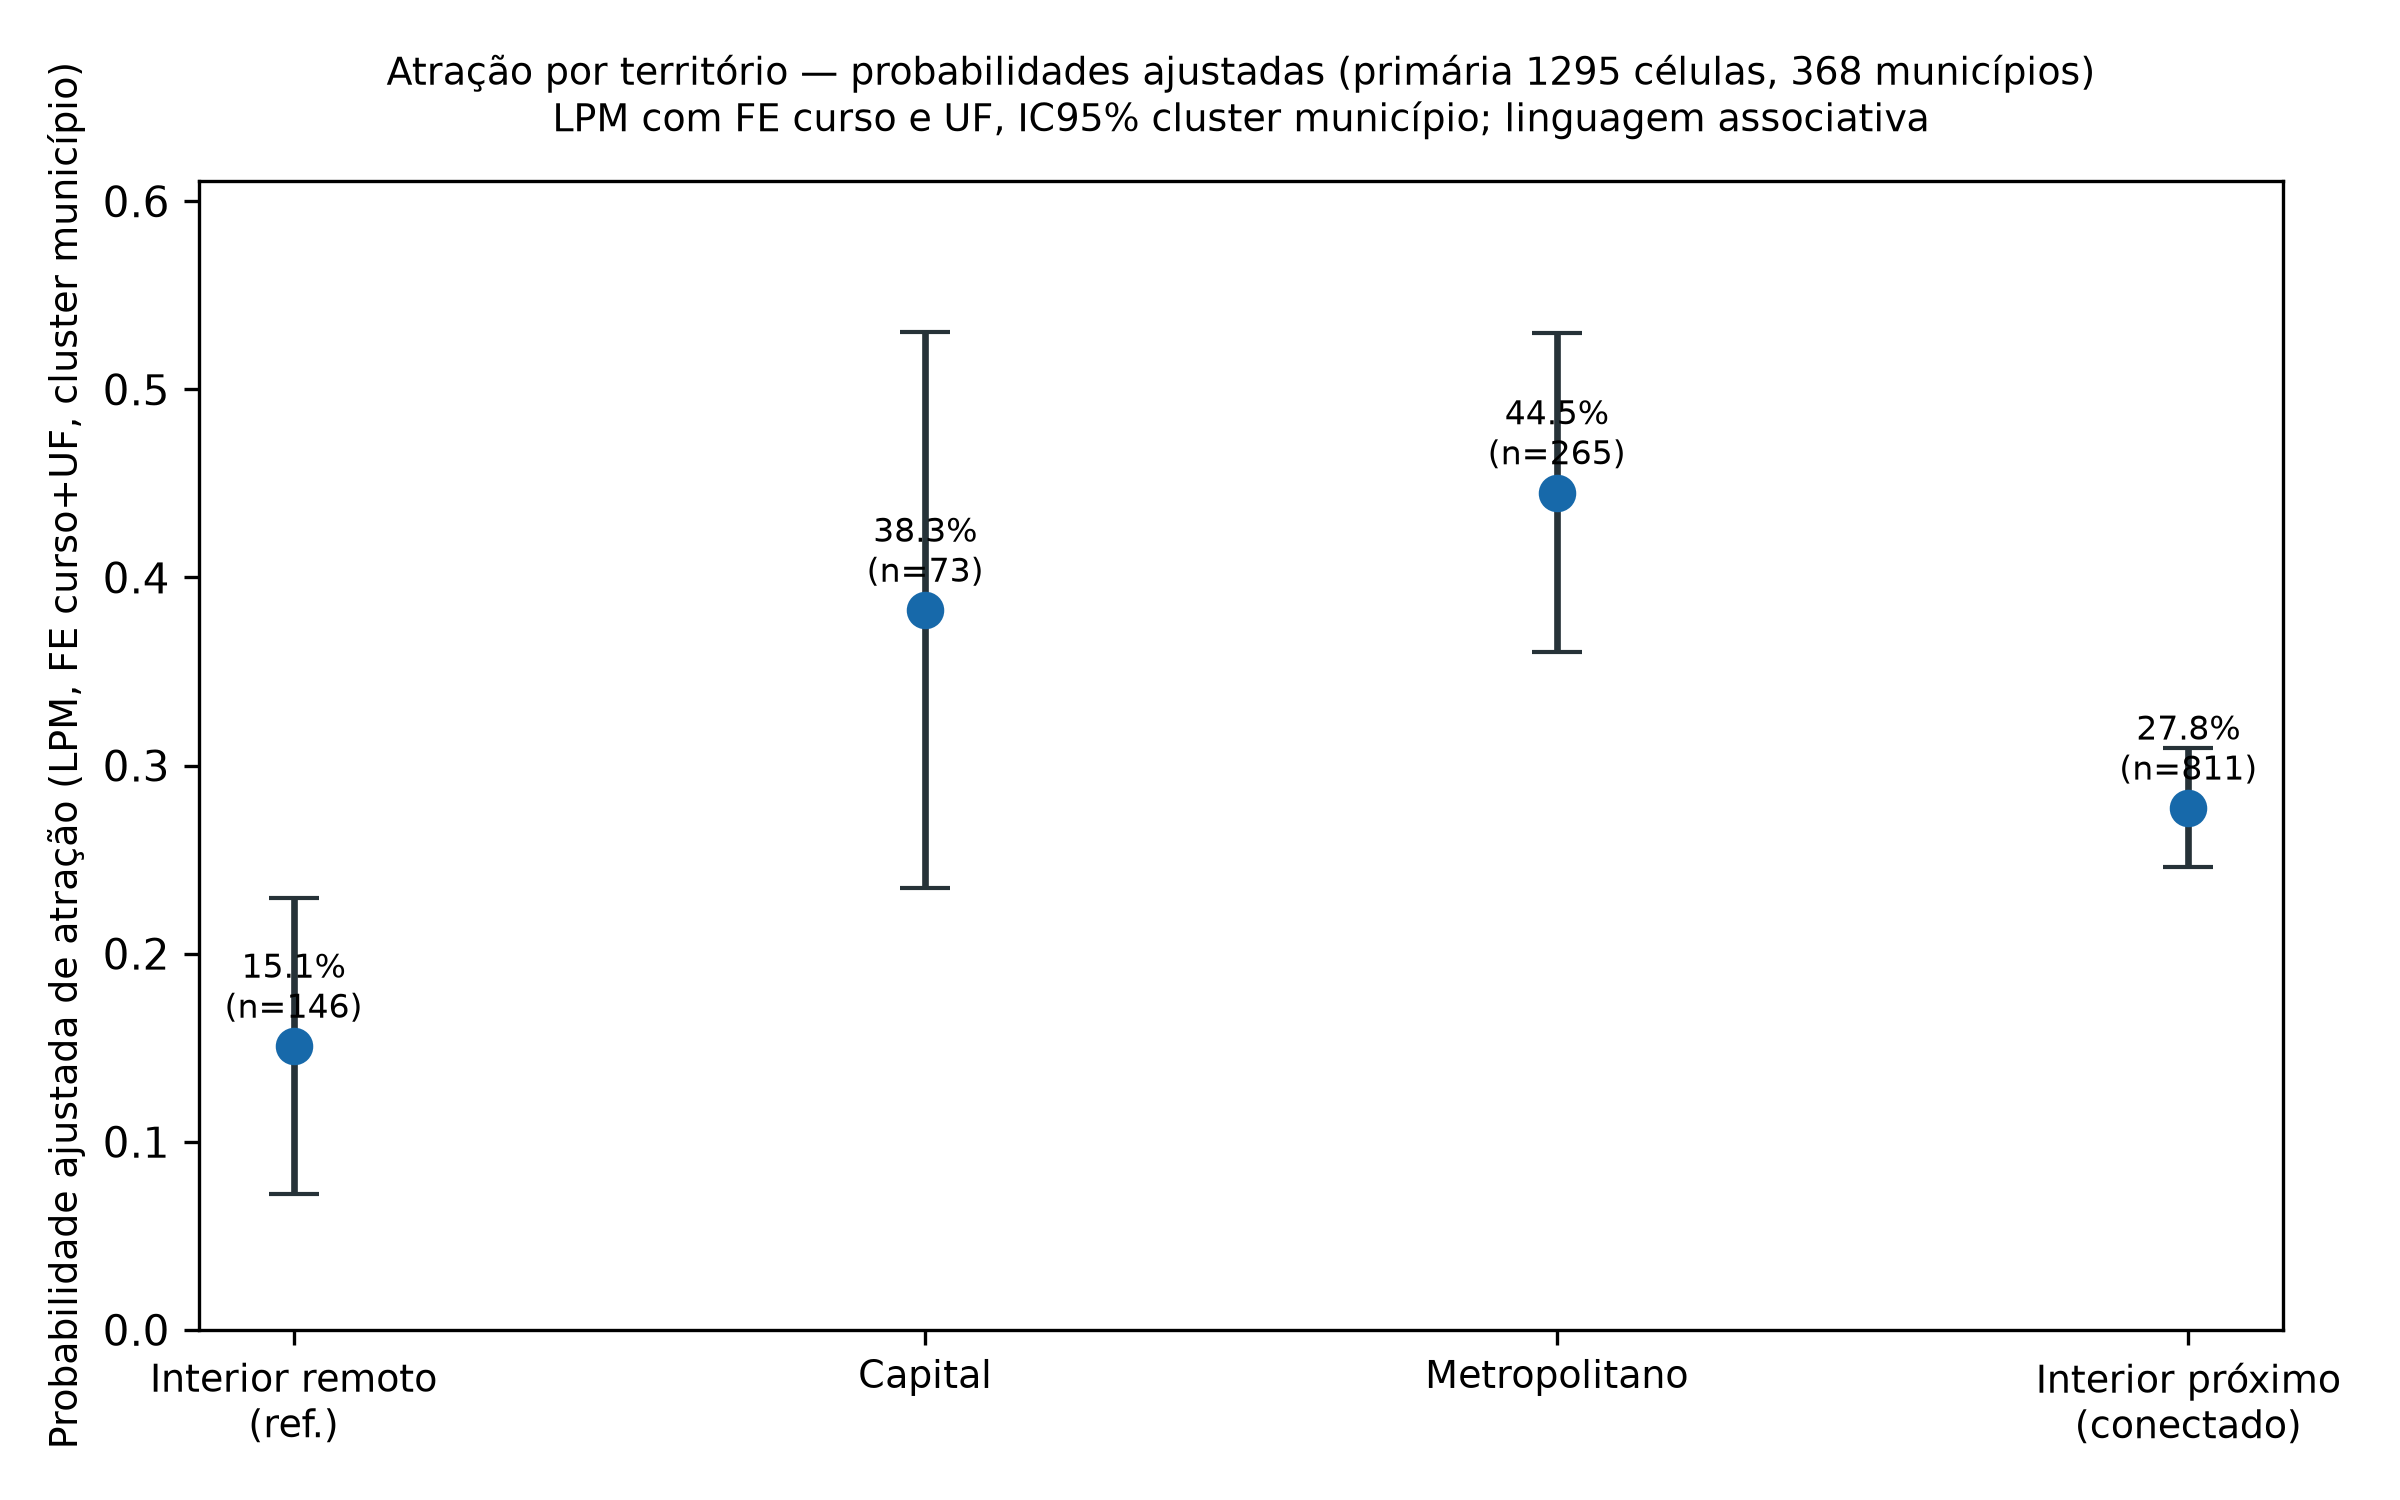
\includegraphics[width=0.9\textwidth]{output/tema_trabalho/A4_figura_01_prob_ajustada_estrato.png}
\caption{Probabilidades ajustadas de atração realizada por estrato territorial.
Intervalos de 95\% usam erros agrupados por município, inclusive para a categoria
de referência. Leitura descritiva.}
\label{fig:a4}
\end{figure}

\section{Evidência associativa: dinâmica do estoque cadastral no CNES}
\label{sec:cnes}

Este apêndice reporta uma análise longitudinal associativa, separada do núcleo
causal e com objeto diferente. Ela pergunta se células município--curso com
atração administrativa apresentaram trajetória distinta de oferta médica
cadastrada, e não se algum profissional específico foi atraído.

Agregamos vínculos do CNES dentro de cada município--curso em 26 competências, de
junho de 2024 a julho de 2026. A amostra confirmatória tem 587 células em 295
municípios, restrita a dez cursos cuja ponte curso--CBO não tem sobreposição.
Junho de 2025 é a última referência inequivocamente anterior à oferta. O desfecho
é o estoque distinto de profissionais cadastrados na célula; ele não identifica
participantes do PMM-E, exercício efetivo nem retenção individual.

O modelo interage a atração realizada com cada competência, omitindo junho de
2025, e absorve efeitos fixos de município--curso, curso--mês e unidade da
federação--mês, com erros agrupados por município. Como atração é um resultado
realizado, e não tratamento atribuído, os coeficientes são diferenças
condicionais de trajetória.

O teste conjunto dos coeficientes anteriores à referência não rejeita zero, com
$F$ de 1,03 e $p$ de 0,420. Em março de 2026, a diferença associada à atração é
de 0,50 profissional por célula, com erro-padrão de 0,23 e $p$ de 0,033. Uma
sensibilidade com as 1.184 células de todos os cursos produz 0,60, com
erro-padrão de 0,22 e $p$ de 0,006, mas mistura CBOs sobrepostos e não é a
amostra principal.

A distribuição da variação entre junho de 2025 e março de 2026 é assimétrica.
Sem atração, a mediana é 0 e a média é 0,55, com máximo de 25; com atração, a
mediana é 1 e a média é 2,29, com máximo de 211. Essa assimetria mostra por que o
resultado precisa ser lido com medianas e caudas, e não apenas com médias.

A Figura \ref{fig:a5} apresenta a trajetória estimada em torno de junho de 2025.

Não rejeitar diferenças anteriores à referência não prova paralelismo, e nada
neste apêndice deve ser usado para reforçar ou confirmar o resultado causal local
da Seção \ref{sec:resultados}: os dois exercícios medem objetos distintos, em
unidades distintas, com estatutos de identificação distintos.

\begin{figure}[htbp]
\centering
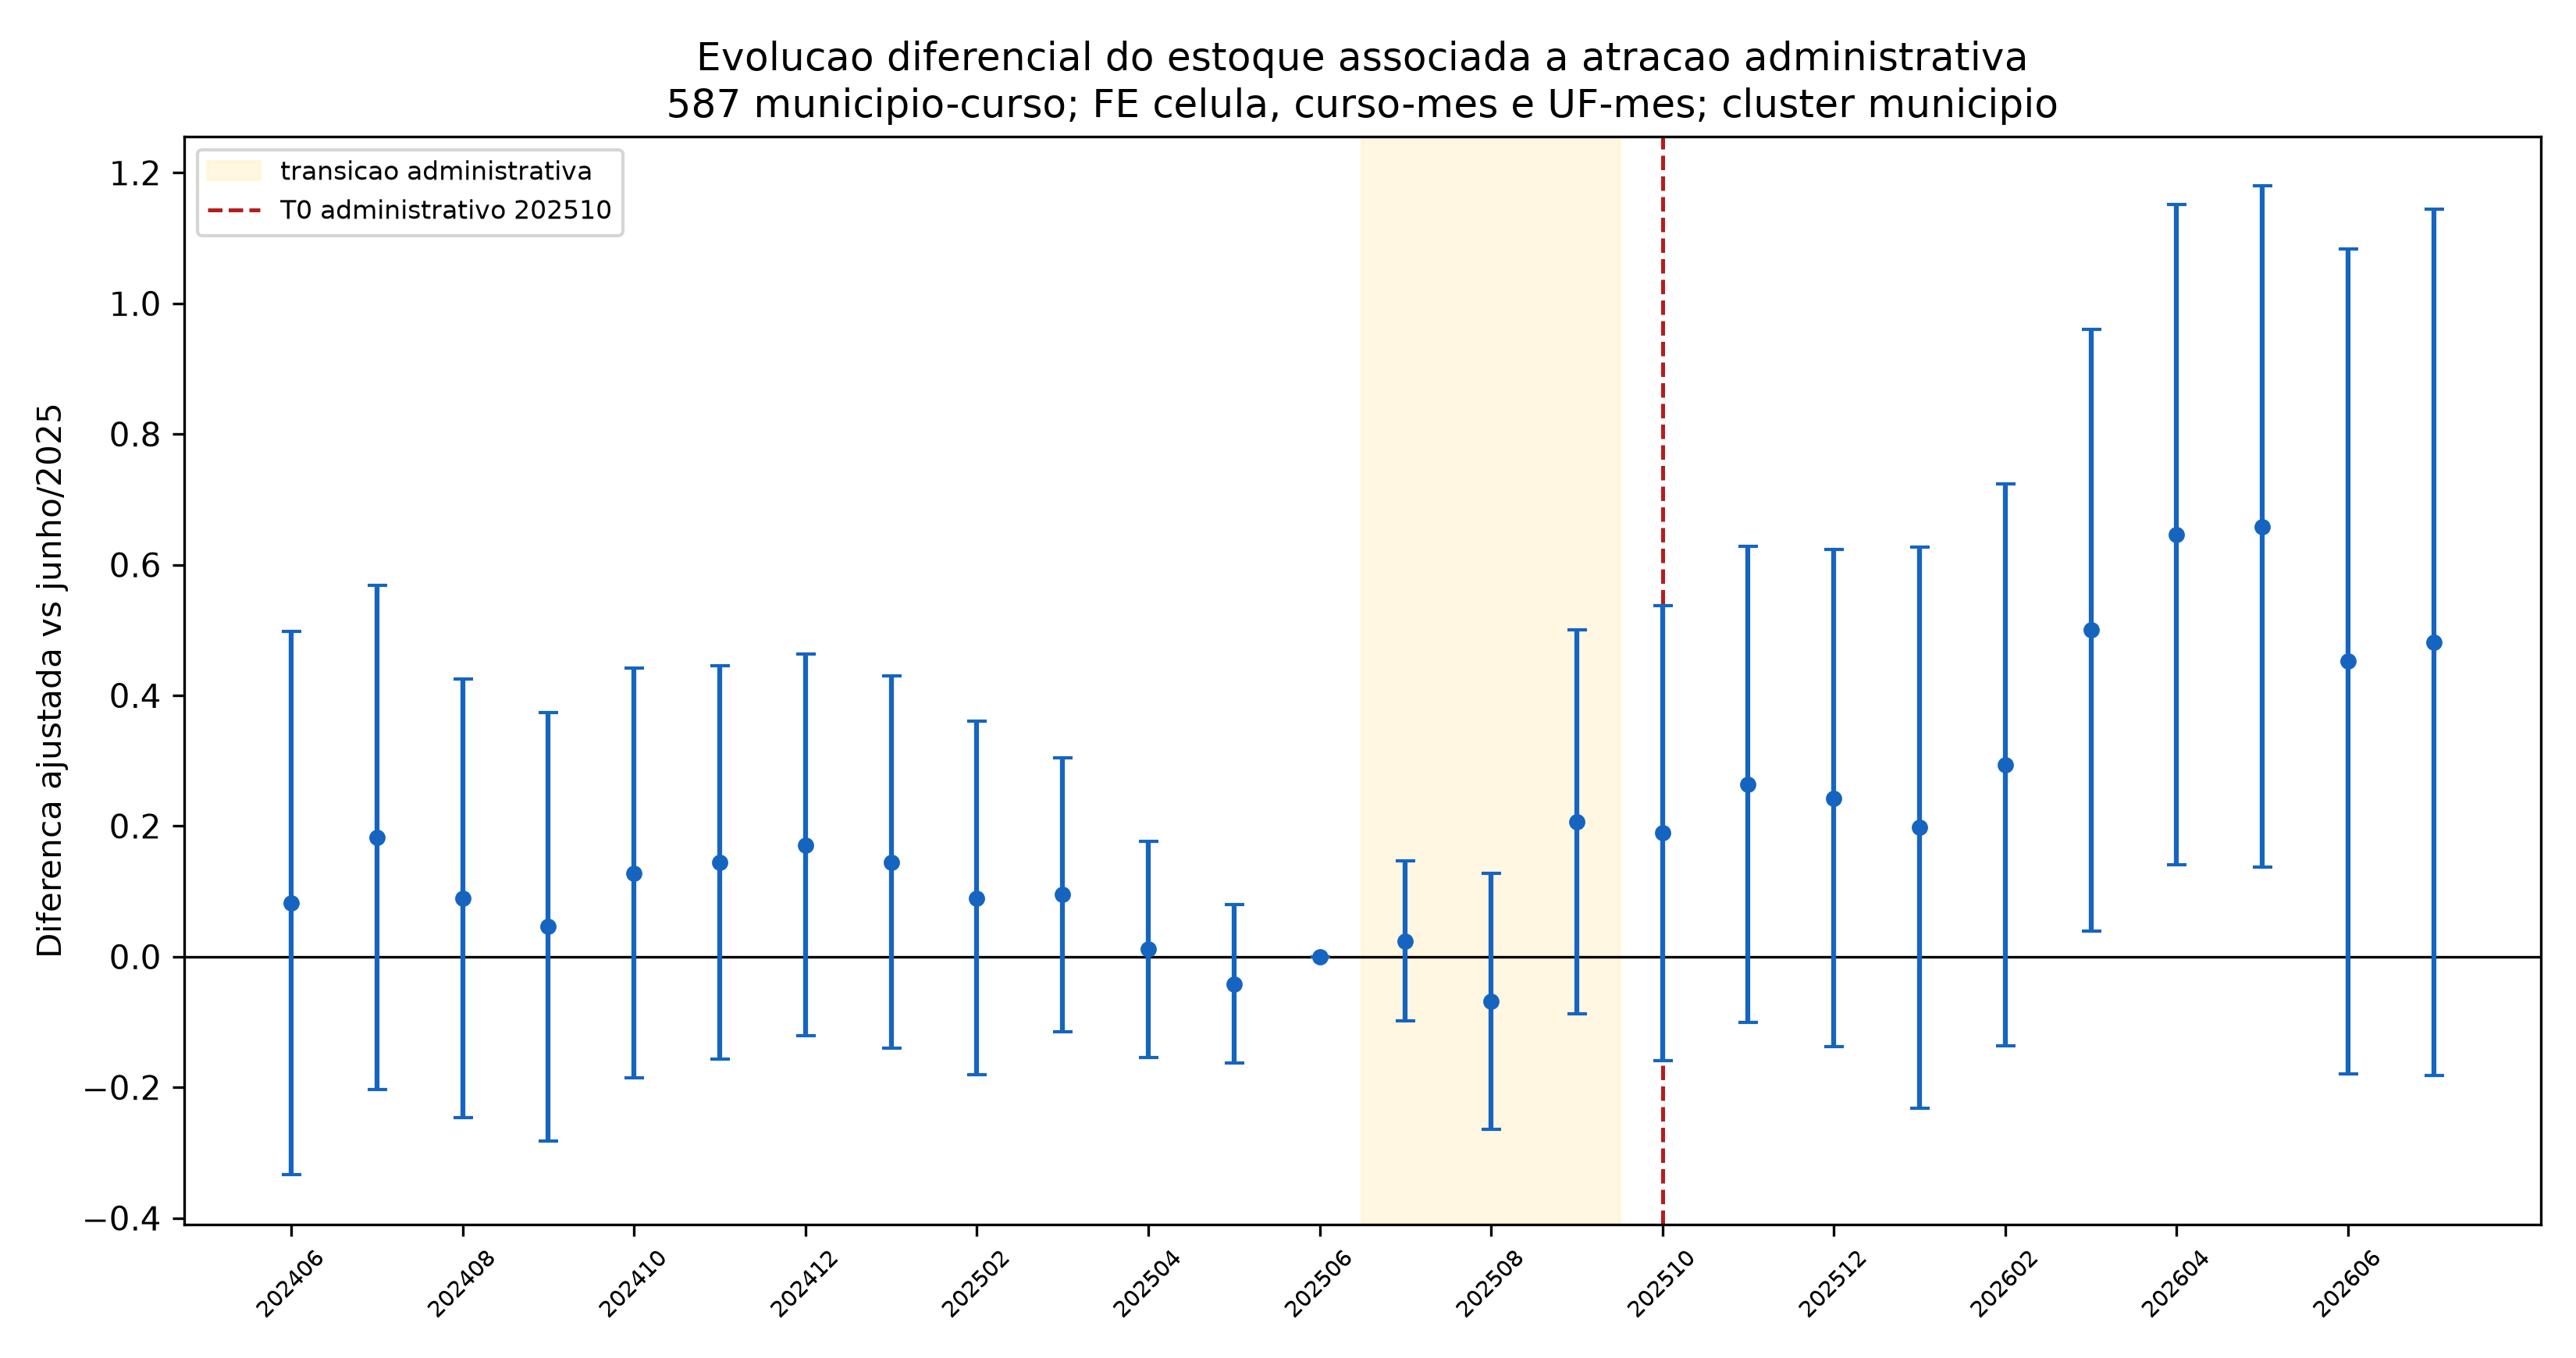
\includegraphics[width=0.94\textwidth]{output/tema_trabalho/A5_figura_04_estudo_evento_atracao.png}
\caption{Evolução diferencial do estoque cadastrado associada à atração
administrativa realizada. Junho de 2025 é a referência. Leitura associativa.}
\label{fig:a5}
\end{figure}

\section{Rotas avaliadas e descartadas}
\label{sec:rotas}

Duas rotas alternativas foram avaliadas antes do desenho adotado e são
registradas aqui como decisões de escopo, e não como resultados.

\textbf{Regressão descontínua do adicional de bolsa pelo IVS.} A faixa de bolsa
anunciada e o IVS 2010 são ligados por regra administrativa, o que sugeriria um
desenho de descontinuidade nos limiares publicados. A auditoria da regra, porém,
não reproduziu a faixa anunciada: aplicando a taxonomia externa ao IVS público,
191 dos 368 municípios são reproduzidos e 177 divergem, ou 48,1\% do total.
Sem regra reproduzível, não há primeiro estágio estável e o desenho foi encerrado
no primeiro portão. O IVS 2010 permanece a \emph{running variable} canônica para
eventual retomada, condicionada à obtenção do escore, da vintagem e da regra
administrativa exatos. Nenhum efeito da bolsa foi estimado neste trabalho.

\textbf{Tripla diferença entre vaga imediata e cadastro de reserva.} Uma
comparação entre células ofertadas para preenchimento imediato e células mantidas
apenas em cadastro de reserva foi avaliada com o estimador de tripla diferença
\citep{olden2022}. No mesmo grão município--curso e na mesma amostra que
identificaria o desenho, com 319 células em 93 municípios, a modalidade imediata
não prediz a alocação confirmada: a diferença ajustada é de 2,79 pontos
percentuais, com erro-padrão de 6,89 pontos percentuais e $p$ de 0,6871. O portão
de relevância não foi aprovado e a rota foi encerrada como comparação ajustada,
sem leitura causal. Cadastro de reserva também não é ausência permanente do
programa e pode receber exposição posterior.

Nenhuma dessas duas rotas contribui com resultados para este artigo. Elas são
reportadas para deixar explícito o conjunto de desenhos considerados e a razão de
cada descarte, evitando a impressão de que o desenho final foi escolhido depois
de comparar estimativas.

\end{document}
